\documentclass[12pt, fleqn, a4paper]{article}
\usepackage[top=2cm, bottom=2cm, left=3cm, right=1.5cm]{geometry}
\setlength{\parindent}{1cm}
\linespread{1.377388535031847}
\usepackage{luacode}


\usepackage{fancyhdr}
\fancyhf{}
\fancyhead[C]{\thepage}
\renewcommand{\headrulewidth}{0pt}
\pagestyle{fancy}

\fancypagestyle{plain}{%
  \fancyhf{}
  \renewcommand{\headrulewidth}{0pt}
  \fancyhead[C]{\thepage}
}


\usepackage{pdfpages}
\usepackage{fontspec}
\defaultfontfeatures{Mapping=tex-text,Scale=MatchLowercase}
\setmainfont{Times New Roman}
\setmonofont{Noto Sans Mono}
\usepackage{indentfirst}
\usepackage{polyglossia}
\usepackage{changepage}
\usepackage[fontsize=12.5pt]{scrextend}
\usepackage{markdown}
\usepackage{etoolbox}
%\usepackage{hyperref,url}
\usepackage{natbib}
\newcounter{bibcount}

\makeatletter
\patchcmd{\@lbibitem}{\item[}{\item[\hfil\stepcounter{bibcount}{\thebibcount.}}{}{}
\setlength{\bibhang}{2\parindent}
\renewcommand\NAT@bibsetup%
   [1]{\setlength{\leftmargin}{\bibhang}\setlength{\itemindent}{-\parindent}%
       \setlength{\itemsep}{\bibsep}\setlength{\parsep}{\z@}}
\makeatother
\bibliographystyle{agsm}


% Настроика qзыкa
\setdefaultlanguage{english}

\usepackage{enumitem}
\setlist[enumerate]{label*=\arabic*.}
\AddToHook{cmd/section/before}{\clearpage}

\usepackage{minted}
\setminted[python]{frame=single}

\usepackage{lipsum}
\usepackage{titlesec}
\renewcommand{\thesection}{\arabic{section}.{}}
\renewcommand{\thesubsection}{\arabic{section}.\arabic{subsection}.{}}
\renewcommand{\thesubsubsection}{\arabic{section}.\arabic{subsection}.\arabic{subsubsection}.{}}

\usepackage{tocloft}
\usepackage{float}
\renewcommand{\cftsecleader}{\cftdotfill{\cftdotsep}} 

\usepackage{sectsty}
\newcommand{\HeaderSize}{\fontsize{14}{15}\selectfont\MakeUppercase}
\sectionfont{\HeaderSize}

\usepackage{chngcntr}
\counterwithin{figure}{section}

\usepackage{xstring}
\def\FixCaptionLabel#1{%
  \IfSubStr{#1}{.}{%
	\StrSubstitute[1]{#1}{.}{}}{#1}}

\usepackage{subcaption}
\DeclareCaptionLabelFormat{custom}
{%
	\FixCaptionLabel{#2}. #1.
}
% Separator style
\DeclareCaptionLabelSeparator{custom}{ }
% Caption format    
\DeclareCaptionFormat{custom}
{%
	#1#2\textbf{#3}
}
\captionsetup
{
    format=custom,%
    labelformat=custom,%
    labelsep=custom
}


\newcommand\signature[2]{% Name; Department
\noindent\begin{minipage}{5cm}
    \noindent\vspace{3cm}\par
    \noindent\rule{5cm}{1pt}\par
    \noindent\textbf{#1}\par
    \noindent#2%
\end{minipage}}

\newcommand\conformationsignature[2]{
\begin{table}[h]
    \begin{tabular}{p{7cm}}
      \\
    \end{tabular}
    \begin{tabular}{p{3cm}}
      \\\hline
    #1 
    \end{tabular}
    \begin{tabular}{p{4cm}}
      \\\hline
    #2 
    \end{tabular}
\end{table}
}

\newcommand\insertdate[1][\today]{\vfill\begin{flushright}#1\end{flushright}}
\usepackage{csquotes}
\usepackage{plantuml}
\usepackage{xcolor}
\definecolor{light-gray}{gray}{0.95}
\newcommand{\codeword}[1]{\colorbox{light-gray}{\texttt{#1}}}
\newcommand{\cw}[1]{\colorbox{light-gray}{\texttt{#1}}}
\newcommand{\boldword}[1]{\textbf{#1}}

\begin{luacode*}
	function split(inputstr, sep)
	        if sep == nil then
	                sep = "%s"
	        end
	        local t={}
	        for str in string.gmatch(inputstr, "([^"..sep.."]+)") do
	                table.insert(t, str)
	        end
	        return t
	end

	function boldenfirstword(line)
		local words = split(line, " ")
		local fword = words[1]
		table.remove(words, 1)
		tex.print("\\textbf{"..fword.."} "..table.concat(words," "))
	end
\end{luacode*}

% declare a wrapper in TeX
\newcommand{\boldenfirstword}[1]{\directlua{boldenfirstword("#1")}}

\usepackage{datatool}
\newcommand{\sortitem}[1]{%
  \DTLnewrow{list}% Create a new entry
  \DTLnewdbentry{list}{description}{\boldenfirstword{#1}}% Add entry as description
}

\newenvironment{sortedlist}{%
  \DTLifdbexists{list}{\DTLcleardb{list}}{\DTLnewdb{list}}% Create new/discard old list
}{%
  \DTLsort{description}{list}% Sort list
  \begin{itemize}%
    \DTLforeach*{list}{\theDesc=description}{%
\item[] \theDesc}% Print each item
  \end{itemize}%
}


\begin{document}
%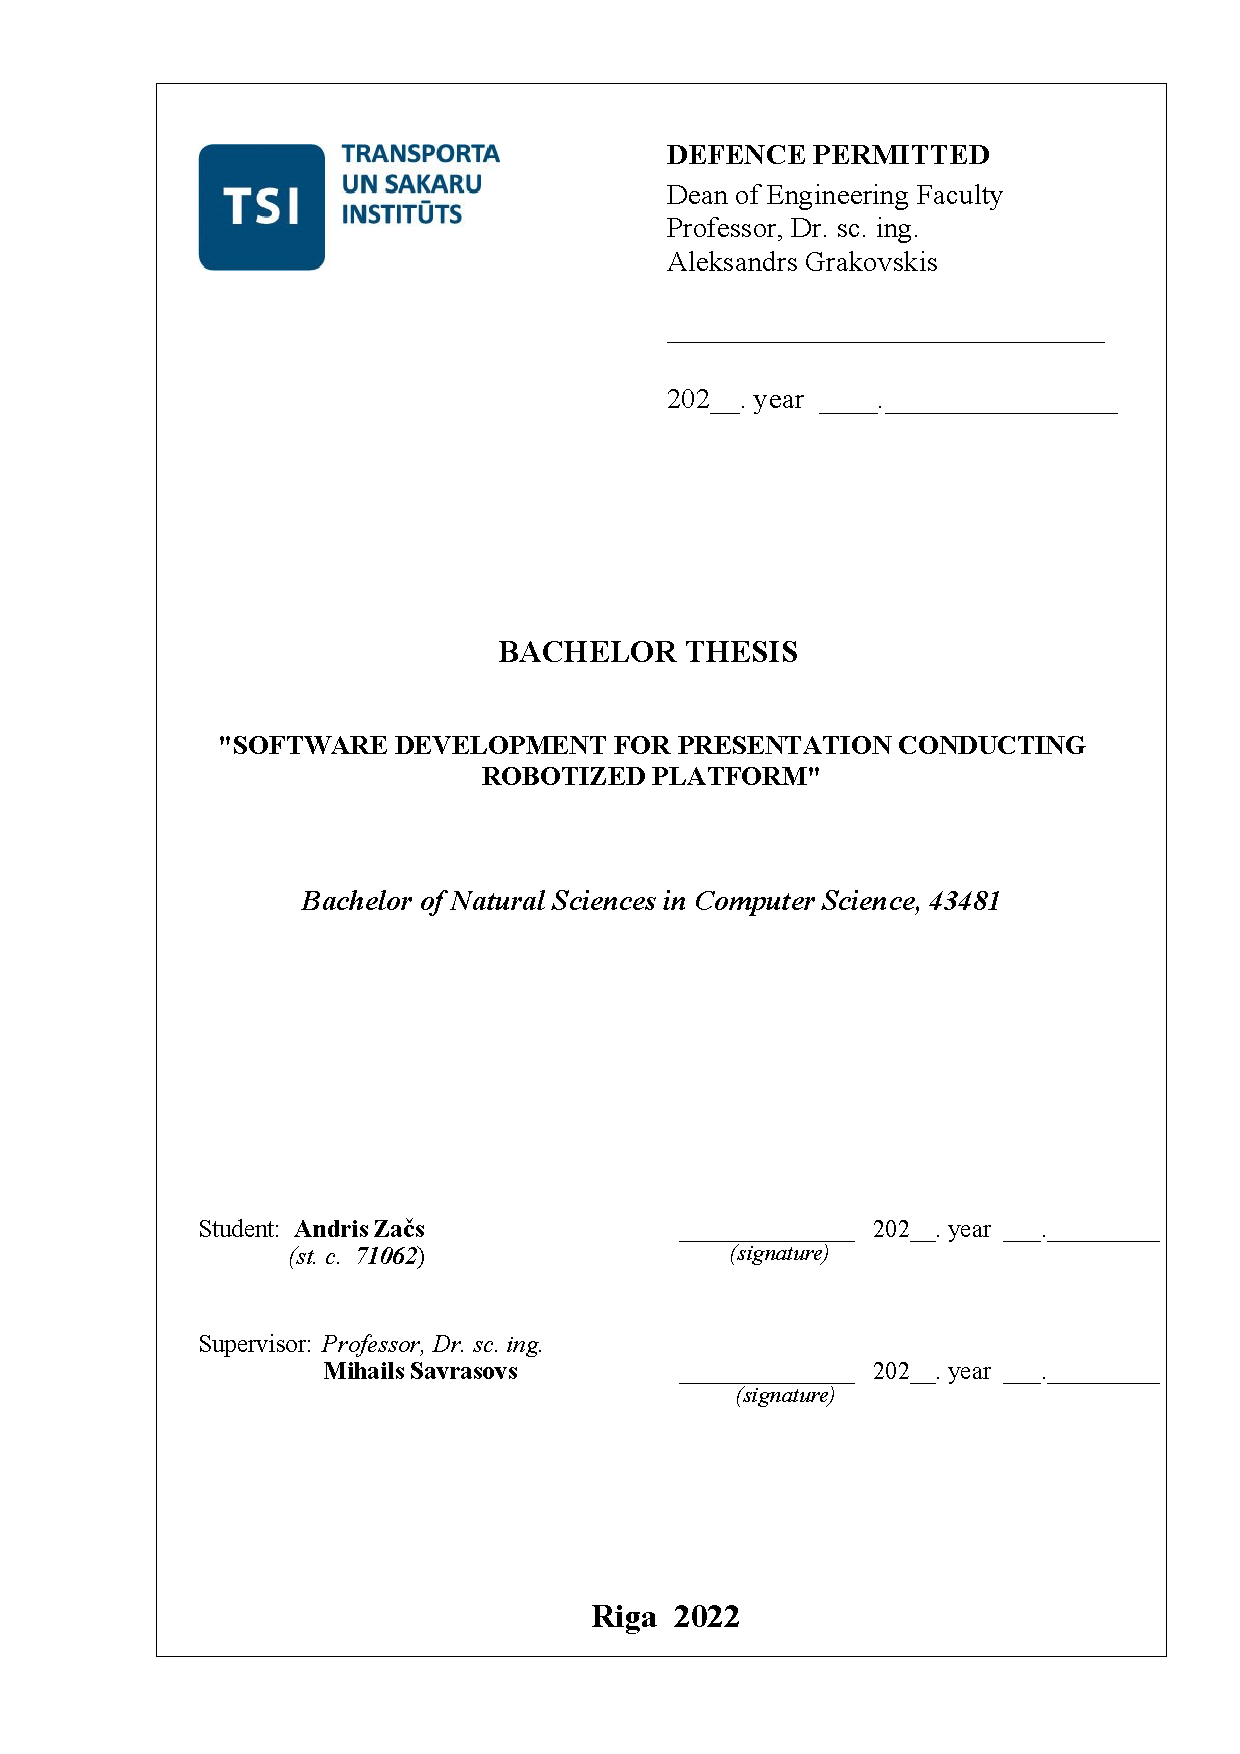
\includepdf[pages={1,2,3,4}]{final.pdf}
\setcounter{page}{5}


\renewcommand{\cfttoctitlefont}{\hfill\Large\bf}
\renewcommand{\cftaftertoctitle}{\hfill\hfill}
\let\oldcontentsname\contentsname
\renewcommand{\contentsname}{ \HeaderSize \hfill \HeaderSize \oldcontentsname}
\renewcommand{\cftsecfont}{\mdseries\scshape\sffamily}
\renewcommand{\cftsecpagefont}{\mdseries\scshape\sffamily}


%\section*{\centering CONFIRMATION}
%I, Andris Začs, confirm that I have developed the given graduation thesis individually for obtaining the degree of Bachelor of Natural Sciences in Computer Sciences. By my signature I verify that the given graduation thesis is written independently and there are no violations regarding the rights of intellectual property of other persons or plagiarism. The used papers and data sources of other authors are indicated in references. The text of the submitted paper has never been submitted partially or fully to other commission for thesis evaluation. I confirm that the electronic version of the submitted thesis meets completely the text of the submitted paper copy of the thesis.
%\\
%\conformationsignature{(signature)}{(name, surname)}
%
%\newpage
%\section*{\centering ABSTRACT}
%Development \enquote{Software development for presentation conducing robotized platform}. Author: Andris Zacs.
%Supervisor: Dr. sc. ing., Mihails Savrasovs.\par
%Paper for obtaining the degree: \enquote{Bachelor of Natural Sciences in Computer Sciences}: X стр., Y рис., Z лит. ист., * прил.\par
%PRESENTATION, ROBOT, NAO\par
%Development of a robotic platform that allows to conduct autonomous interactive presentations using the Nao robot, with the ability to interact with the robot in real time and also the ability to interact with the audience through polls.
%For interfacing with Nao, a program was developed with a convenient and intuitive UX design.
%The system was implemented in Python using the public SDK for Nao - qi framework, Django web framework and PyQt GUI framework.
%As a result, 3 Python programs were developed.
%\newpage
%\section*{\centering АНОТАЦИЯ}
%Разработка \enquote{Разработка модуля для процедурной генерации 3D моделей
%растений}. Автор работы: Андрис Зачс.
%Научный руководитель: Dr. sc. ing., Михаил Саврасов.
%Работа на соискание степени: \enquote{Бакалавр естественных наук в области компьютерныхнаук}: X стр., Y рис., Z лит. ист., * прил.\par
%ПРЕЗЕНТАЦИЯ, РОБОТ, NAO\par
%Разработка роботизированной платформы позволяюшая автономно проводить интерактивные презентации при помощи робота Nao, с возможностью взаимадествия с роботом в реальном времени и также возможностью взаимодейтвий с аудиторией посредством опросов. 
%Для раборы с Nao была разработана программа с удобным и интуитивно понятным UX дизайном.
%Работа реализованна на языке Python, используя общедоступный SDК для Nao qi фреймворк, веб фреймворк Django и GUI фреймворк PyQt.
%В результате былo написано 3 Python программы.
%\newpage
%\section*{\centering ANOTĀCIJA}
%Izstrāde “Programmatūras izstrāde prezentācijas vadīšanai robotizētai platformai”. Autors: Andris Zacs. Darba vadītājs: Dr. sc. ing., Mihails Savrasovs.\par
%Referāts grāda iegūšanai: “Dabaszinātņu bakalaurs datorzinātnēs”: X стр., Y рис., Z лит. ист., * прил.\\
%PREZENTĀCIJA, ROBOTS, NAO.\par
%Robotizētas platformas izstrāde, kas ļauj vadīt autonomas interaktīvas prezentācijas, izmantojot Nao robotu, ar iespēju mijiedarboties ar robotu reāllaikā un arī iespēju ar aptauju palīdzību mijiedarboties ar auditoriju. Saskarsmei ar Nao tika izstrādāta programma ar ērtu un intuitīvu UX dizainu. Sistēma tika ieviesta Python, izmantojot publisko SDK for Nao - qi framework, Django tīmekļa ietvaru un PyQt GUI ietvaru. Rezultātā tika izstrādātas 3 Python programmas.
%\newpage


\setlength\cftbeforesecskip{1pt}

\tableofcontents
\newpage

\addcontentsline{toc}{section}{List Of Used Abbreviations}
\section*{\centering List Of Used Abbreviations}
\begin{adjustwidth}{113pt}{43pt}
	\begin{sortedlist}
		\sortitem{NPTS - Nao Presentation Tool Suite}
		\sortitem{API - Application Programming Interface}
		\sortitem{VCS - Version Control System}
		\sortitem{IP - Internet Protocol}
		\sortitem{XML - Extensible Markup Language}
		\sortitem{SDK - Software Development Kit}
		\sortitem{IPC - Inter Process Communication}
		\sortitem{COM - Component Object Model}
		\sortitem{CLSID - Class Identifier}
		\sortitem{STA - Single-threaded apartment}
		\sortitem{MTA - Multi-threaded apartment}
		\sortitem{SSH - Secure Shell}
		\sortitem{CI - Continuous Integration}
		\sortitem{PPTX - PowerPoint Open XML}
		\sortitem{UX - User Experience}
		\sortitem{HTTP - Hypertext Transfer Protocol}
		\sortitem{AWS - Amazon Web Services}
		\sortitem{DTL - Django Template Language}
		\sortitem{HTML - Hyper Text Markup Language}
		\sortitem{CSS - Cascading Style Sheets}
		\sortitem{XSD - XML Schema Definition}
		\sortitem{JSON - JavaScript Object Notation}
	\end{sortedlist}
\end{adjustwidth}
\addcontentsline{toc}{section}{Introduction}
\section*{\centering Introduction}
Robotics is a rapidly developing branch of engineering. In order to demonstrate its capabilities, a French robotics company developed Nao. A programmable autonomous humanoid robot. It was created for the purposes of research, education and entertainment. As an extension of this idea, a tool suite was developed with which one can make Nao do presentations.\\
Nao Presentation Tool Suite (NPTS) consists of mainly 3 modules:
\begin{itemize}
	\item Nao presentation controller program;
	\item Nao GUI shell;
	\item Survey conductor.
\end{itemize}\par
Nao presentation controller program is mainly responsible for opening a presentation, making the robot Nao read out the text for each slide and jumping to the next slide. In addition, it is capable of playing embedded audio/video and to hold a survey by interfacing with the Survey conductor. The audible for text each slide is provided in the notes section. \par
Nao GUI shell is meant to simplify the users' workflow by providing an intuitive user experience through which one may interact with Nao, configure him and launch the presentation controller program.\par
Survey conductor is a bare web application that can be used to hold surveys. User is meant to provide a PIN through which they are forwarded to a multiple choice survey. Said survey is created and started by the presentation controller program. The interaction between the survey conductor and presentation controller happens through a simple web API.\par
There exists an available market alternative, known as \enquote{NAO Presenter application} which in many ways fulfills the same purpose, aside from some minor differences in the technical implementations and intended use cases. Additionally, \enquote{NAO Presenter application} was created as a business-to-business application solution and most definitely not for an individual persons use and according to its creators it was designed for organizations that receive the public, e.g.
\begin{itemize}
	\item Museums;
	\item Shopping centers;
	%\item Shows;
	\item Civic offices;
	\item Company reception areas.
\end{itemize}
In all other parameters, there seems to be little difference between \enquote{NAO Presenter application} and NPTS. \par
The development of NPTS was a cooperative effort undertaken by 2 individual students. Work was evenly distributed between them. A concrete work breakdown structure will be provided later on. Since the development phase was a team effort, many measures were put in place in order to ensure a smooth workflow, such as a VCS, Kanban Board, Continuous integration pipeline, automated code linting and quality inspection.
\section{Development Objectives}
From the very beginning, a number of objectives and criteria were established for the end product, so that it will have all the required features to be realistically useful and usable.
\subsection{Nao presentation controller}
Upon starting the Nao presentation controller, the program will be able to accept the following input arguments:
\begin{itemize}
	\item Path to a PPTX file;
	\item IP address for a Nao robot;
	\item flag to indicate internet usage (internet usage is required in case a survey is held).
\end{itemize}
The program launches PowerPoint and starts a slide show for the inputted PPTX file. If the program is unable to find the PPTX file or to connect to Nao, an error is raised and the program exits. In case no errors are raised, each slide is sequentially presented to the audience. The text that is read out by Nao is specified in the notes for each slide. In addition to audible words, in the notes there may also be commands that are executed during the reading. These commands may be to:
\begin{itemize}
	\item Execute an animation;
	\item Raise/lower voice volume;
	\item Pause the speech for a certain amount of seconds;
	\item Trigger the next slide animation;
	\item Set a reading mode;
	\item Start playing the embedded media object on the current slide;
	\item Create/start survey.
\end{itemize}
A somewhat unified ad-hoc syntax was developed for these commands. The commands will visually look similar to XML tags. However, this visual resemblance is completely superficial. There tags for the most part, are not used to describe or define elements withing the text but rather to signify commands to execute during the speech. 
Their visual resemblance to XML is mainly used to signify to the reader/writer of the notes that the commands are not part of the speech and are inaudible.\par
The program goes forward slide by slide, until it reaches the end and then closes the slide show and PowerPoint along with it.
\subsection{Nao GUI shell}
Nao GUI shell is meant to give a pleasant user experience and enable the user to more comfortable interact with Nao to perform, for example, administrative or maintenance tasks. In addition, it is meant to supplement the presentation controller by being able to validation a presentation and it's notes and to help a user design surveys for the presentations without burdening the user with any XML-like text blobs.\par
Since this is an application with a graphical interface, some sort of GUI toolkit is necessary. PyQt framework will be used because:
\begin{itemize}
	\item Comes with a litany of complete and ready UI components;
	\item Is well-supported and has many available learning resources;
	\item Is easy to learn and use;
	\item Enables writing a smoother codebase.
\end{itemize}
In addition, some SSH related libraries will be used to help establish a secure and stable connection to the Nao robot.
\subsection{Survey conductor}
The survey conductor is a web application that is meant to be publicly accessible to members of the audience. During the presentation, a survey may be created and started by the presentation conductor. Upon creation, all the questions and answer choices must be provided along with a time limit for each question and also a PIN code must be set by which the audience members will be able to access the survey.\par
The presentation controller may send a request to start it. The survey conductor then autonomously holds the survey by waiting for the time limit for the question to run out and switching to the next one. After the last question expires the survey is closed and no more interaction is possible with it.\par
No data processing or aggregation will be conducted. All of the created surveys are essentially stored in memory and not saved or persisted to any storage medium.
\subsection{Work breakdown structure}
The development of the Nao Presentation Tool Suite was a cooperative endeavor and as such, responsibilities and tasks had to be delegated. Development of the survey conductor and presentation controller was given to one and the rest to the other. A work breakdown structure diagram was conceived to properly visualize this.
\begin{figure}[H]
	\centering
	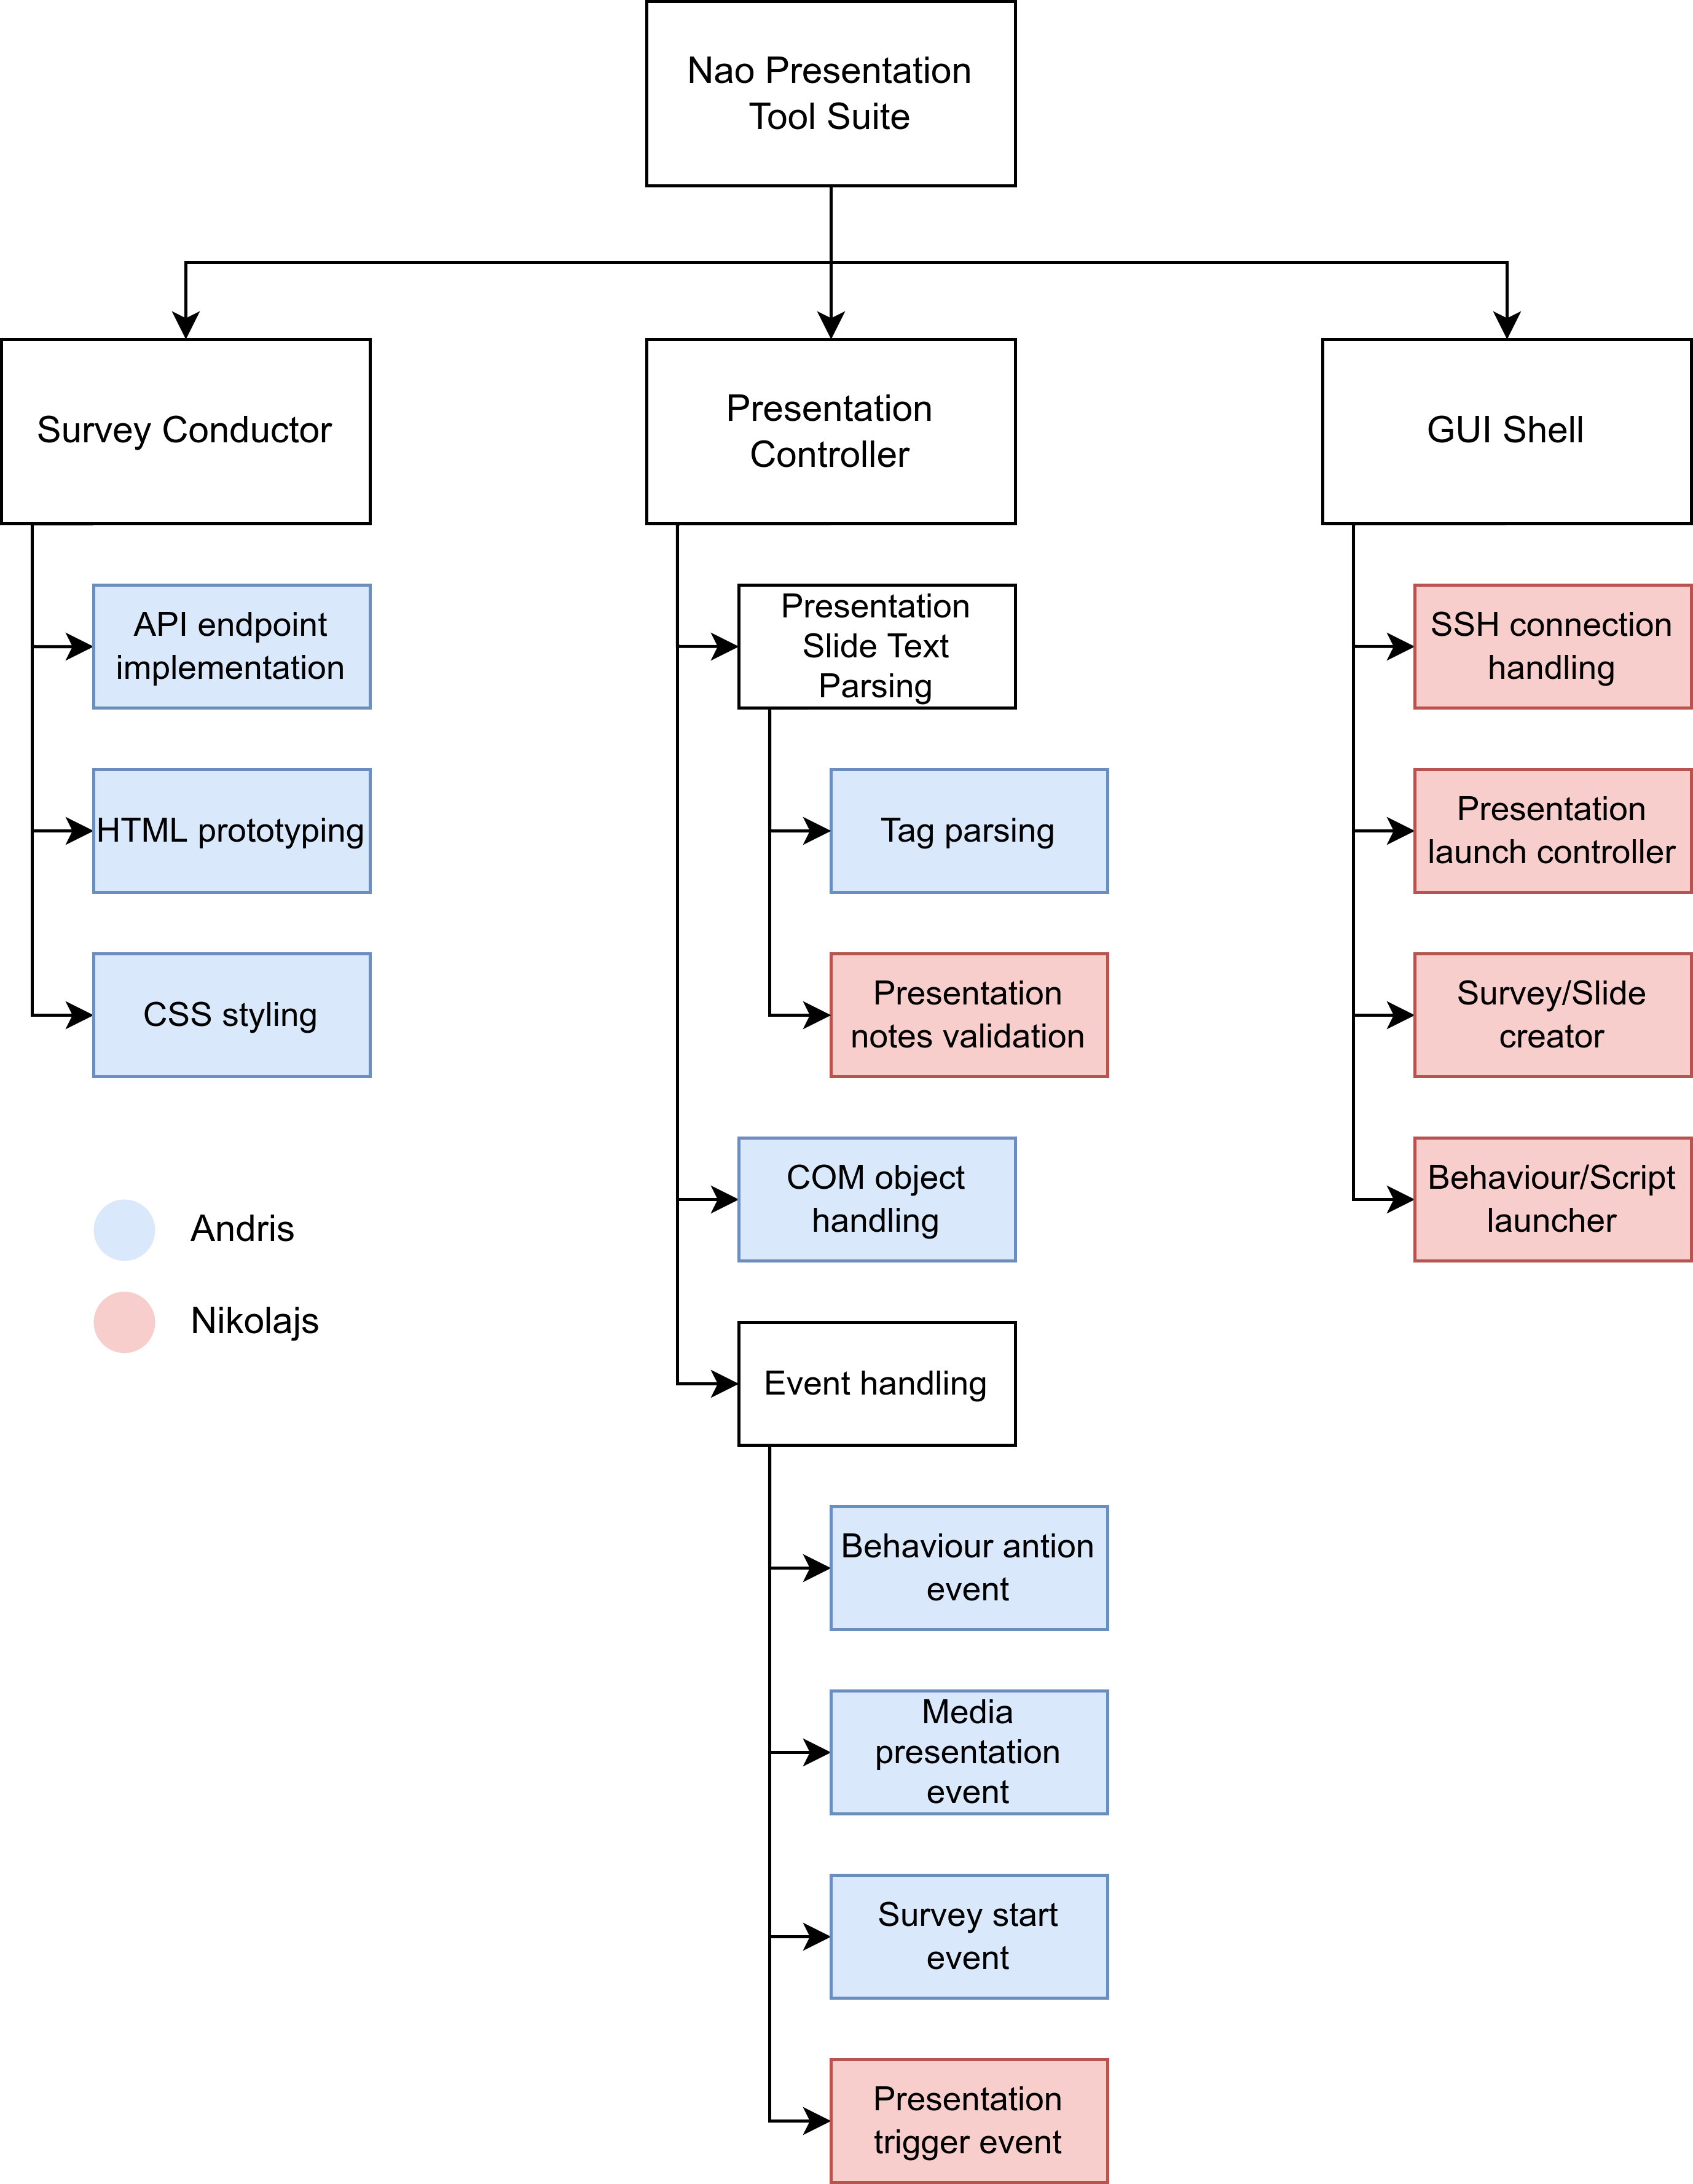
\includegraphics[width=1\textwidth]{img/wbs2.png}
	\caption{Work breakdown structure for the development}
\end{figure}

\section{Design Engineering} % проектирование
In order to successfully develop the tool suite as per all the above stated requirements and criteria, many decision and design choices had to be made in advance.
\subsection{Nao robot}
Nao is an autonomous, humanoid robot that can be programmed with the Qi framework - an easy to use, highly abstracted SDK that enables a novice programmer to write advanced software without getting involved with any low-level hardware concepts like switch debouncing and to quickly and simple utilize all of its motors and sensors, of which it has many.
\begin{figure}[H]
	\centering
	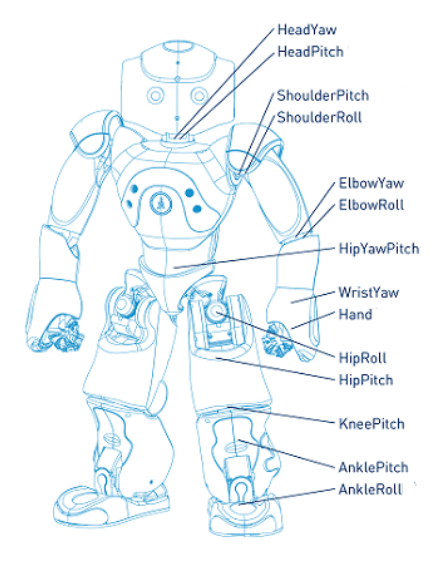
\includegraphics[width=0.75\textwidth]{img/nao.png}
	\caption{Locations of Nao's motors}
\end{figure}
Nao runs a custom Linux distribution. One can connect to it through SSH to debug issues, conduct certain administrative tasks or as a means to study it more thoroughly. An Apache HTTP server instance is also running on Nao, can be reached by using a web browser and used to perform some simple configurations:
\begin{itemize}
	\item Setting voice;
	\item Raising/lowering speech volume;
	\item Configuring Wi-Fi networks.
\end{itemize}
\par
In the context of the Nao presentation tool suite, Nao is used mainly as a speech synthesizer. The main advantage that Nao has over other text to speech services is its ability to supplement speech with movements and gestures making it much more expressive and effective as a presenter.
The following modules of the Qi framework were used during development:
\begin{itemize}
	\item ALTextToSpeech - used to make Nao talk using the text-to-speech engine.
	\item ALAnimatedSpeech - makes Nao speak in an expressive manner.
	\item ALAutonomousLife - module that is used to configure Nao's autonomous behavior.
	\item ALSpeechRecognition - module used to configure Nao's speech recognitions patterns.
	\item ALTouch - module used to read state of Nao's sensors.
	\item ALMemory - allows acceess to Nao's centralized memory, which is used to store Nao's hardware configuration and other vital information.
	\item ALRobotPosture - module allows to make Nao go to different predefined postures.
	\item ALBehaviorManager - module to manage behaviors. A behavior being a set of instructions that can be installed on Nao.
\end{itemize}
\subsection{COM objects}
In order facilitate the interaction between the presentation controller program and PowerPoint it was decided that COM objects will be used, as it appears to be the most reliable and secure method of IPC for when it comes to Microsoft Office Applications \citep{stevewhims}. If PowerPoint is installed on a system, it registers itself, and it's CLSID into the system's registry. It is then possible to create a new object instance in a language such as Python and call upon this object various methods to orchestrate a slide show. It should be noted that every office application technically has its own object model, but due to the efforts of Microsoft the object model has become fairly similar between all the applications, making the learning curve much lower.\par
\begin{figure}[H]
	\centering
	\begin{plantuml}
@startwbs
* Application
** Presentation
*** Slide Master
*** Slides (collection)
**** Slide
**** Shapes (collection)
***** Title
***** Shape
****** TextFrame
****** Table
****** Diagram
@endwbs
	\end{plantuml}
	\caption{PowerPoint object model \citep{ppmodel}}
\end{figure}
The API for each COM object type is well documented and described in the official and publicly available Microsoft docs and also some books \citep{box1998essential}. For the purposes of conducting a presentation the following objects were used:
\begin{itemize}
	\item Application object (PowerPoint), utilizing:
		\begin{itemize}
			\item Method Open - accepts absolute file path to a PPT/PPTX file;
			\item Method Quit - exits PowerPoint.
		\end{itemize}
	\item Presentation object, utilizing:
		\begin{itemize}
			\item Property SlideShowSettings - object which represents the slide show settings for the opened presentation;
			\item Method Close - closes the specified presentation.
		\end{itemize}
	\item SlideShowSettings object, utilizing:
		\begin{itemize}
			\item Method Run - runs a slide show of the opened presentation returning a SlideShowWindow object.
		\end{itemize}
	\item SlideShowWindow object, utilizing:
		\begin{itemize}
			\item Property View - SlideShowView object;
			\item Method Exit - exits the slide show.
		\end{itemize}
	\item SlideShowView object, utilizing:
		\begin{itemize}
			\item Method GotoSlide - accepts integer value indicating which slide to go to;
			\item Property Slide - object representing the currently selected slide;
			\item Method Player - accepts ID for Shape object and returns Player object instance.
		\end{itemize}
	\item Slide object, utilizing:
		\begin{itemize}
			\item Property Shapes - a collection representing all elements placed on slide.
		\end{itemize}
	\item Shape object, utilizing:
		\begin{itemize}
			\item Property ID - number that uniquely identifies the shape object;
			\item Property Type - number indicating type of element (Number 16 stands for embedded media).
		\end{itemize}
	\item Player object, utilizing:
		\begin{itemize}
			\item Method Play - starts playback for specified media.
		\end{itemize}
\end{itemize}
\subsubsection{COM in multithreaded applications}
The execution of commands (for media playback for example) happen concurrently with the main process thread. However, when it comes to multithreaded usage of COM objects there are some pitfalls that should be avoided.\par
COM has a very long history in Windows. It existed as far back as 16-bit Windows where each process had only one thread. So much of the component object model was designed and written under the assumption that it would be running in a single-threaded application. When Windows NT introduced multithreading, a limitation was initially imposed upon COM objects. A COM object could only be used on the thread that it was created on. In other words, each thread was treated as a single-threaded pseudo process, later dubbed (STA) \enquote{Single-threaded apartment} \citep{chen_2019}.\par
The only way to effectively use the same COM object on different threads was by marshalling it across, i.e.\ marshalling the COM object into an ID on the parent thread, relaying that ID to another thread and then unmarshalling the ID back into a COM object. Initially, the presentation controller was designed and developed around this concept.\par
Some time later, COM introduced the concept of \enquote{Multi-threaded apartments} (MTA) in which one can freely use objects among different threads without marshalling. A thread can opt into the MTA by padding \codeword{COINIT\_MULTITHREAD} flag to function \codeword{CoInitializeEx} \citep{pywin32}. Once this was discovered, presentation controller was redesigned and rewritten to utilize MTA.
\begin{figure}[H]
	\centering
	\begin{plantuml}
@startuml
package Process {
  package "STApartment " {
    rectangle "Thread    " 
    rectangle "COM Object 3"
  }
  package STApartment {
    rectangle "Thread " 
    rectangle "COM Object 1"
  }

  package MTApartment {
    rectangle "Thread  "
    rectangle "Thread   "
    rectangle "COM Object 2" 
    
  }
}
[COM Object 2] <-up-> [Thread  ]
[COM Object 2] <-up-> [Thread   ]
[COM Object 1] <-up-> [Thread ]
[COM Object 3] <-up-> [Thread    ]
'[COM Object 1] <-[norank,dashed,#ff0000]-> [Thread    ]

@enduml
	\end{plantuml}
	\caption{COM threading model}
\end{figure}
\subsection{Programming Language}
In order to rapidly develop applications for Nao, the official SDK was used, which narrows the choice between mostly only 2 programming languages: C++ or Python. Older version of the SDK also had support for \verb|.Net|, Java, JavaScript and Matlab, however these appear to no longer be officially supported.\par
It was deemed that C++ would be a poor fit for the following reasons:
\begin{itemize}
	\item Application does not have serious CPU performance requirements. No intense computations will be taking place and as such there is no need for granularity or optimization that C++ permits to the developer.
	\item Inexperienced use of C++ that involves making use of OOP features like classes and objects, almost always leads to memory leaks. Even more so when development is being done by more than one person.
	\item Using COM objects in C++ is fairly inconvenient. COM objects are utilization is much more effective with dynamic languages such as Visual Basic or Python.
\end{itemize}
For these reasons Python was chosen for development. Since the Nao SDK does not support the latest major version of Python (Python 3), Python 2 will be used for developing the Nao presentation controller. 
In all other cases, Python 3 will be used because it:
\begin{itemize}
	\item Supports type hinting, which, when utilized, makes the source code more reliable, readable and maintainable.
	\item Has a slightly more comprehensive and readable syntax.
	\item Has more new features and operators:
		\begin{itemize}
			\item Walrus operator;
			\item String interpolation (f-strings);
			\item Switch/Case expressions;
			\item Better and more descriptive error messages;
		\end{itemize}
	\item Is officially supported and will be patched in cases when vulnerabilities are discovered.
\subsubsection{Python IDE}
To make the development process smoother, a proper feature-rich integrated development environment can go a long way. For this reason, PyCharm was selected and used. It provides many helpful features such as:
\begin{itemize}
	\item Live code validation and syntax highlighting;
	\item support for plugins like sonarlint which help in some cases to immediately identify and resolve semantic code issues;
	\item allows debugging python code without any external requirements;
	\item ability to quickly and easily set up and change the default python interpreter for a project.
\end{itemize}
The only noteworthy disadvantage for PyCharm, being its slow loading time.
\end{itemize}
\subsection{Methodology}
Since the development of the Nao presentation tool suite would be a collaborative effort, certain measures, methods and methodologies had to be employed in order to ensure a smooth and frictionless workflow.
\subsubsection{Kanban}
For the efficient distribution of tasks a Kanban board was created on GitHub. This board is a project management tool meant to help visualize the state of development and maximize efficiency \citep{degrandis_demaria_2017}. The created Kanban board had 3 columns:
\begin{itemize}
	\item To do;
	\item Work in Progress;
	\item Complete.
\end{itemize}
\begin{figure}[H]
	\centering
	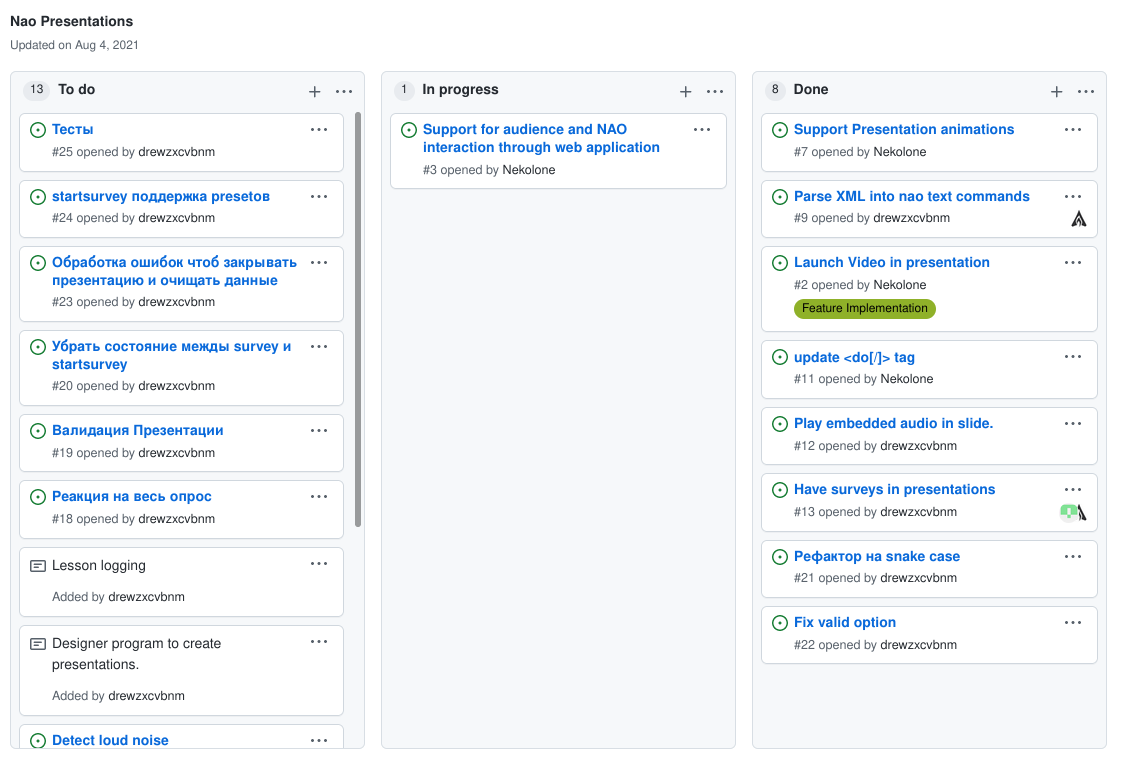
\includegraphics[width=0.9\textwidth]{img/kanban_board.png}
	\caption{Snapshot of the kanban board during development}
\end{figure}

\subsubsection{Version Control System}
A version control system is a necessity for all pretty much all software development projects. It enables developers to work collaboratively and safely. With it developers can synchronize their changes with one another and efficiently resolve conflicting code changes \citep{loeliger_mccullough_2012}.\par
For the development of the presentation tools suite, Git and GitHub were used. 
Git can be thought of as a database to store snapshots of the codebase throughout its development phase. At the core of Git is a key-value data store. 
There are 3 main types of objects that git stores \citep{progit}:
\begin{itemize}
	\item Blob: used to store file contents
	\item Tree: stores file directory structure
	\item Commit: contains within itself a reference to a Tree object and possibly references to one or two parent commits.
\end{itemize}
It supports many useful features for development:
\begin{itemize}
	\item Version branching;
	\item Great Scalability;
	\item Distributed development.
\end{itemize}
In addition, GitHub, git's most popular repository hosting service, also provides many significant advantages:
\begin{itemize}
	\item Secure remote repository access control;
	\item Kanban board creation;
	\item Continuous Integration pipeline support;
	\item Git branch access control;
	\item Branch Merge Requests.
\end{itemize}
By utilizing GitHub's many features, a secure and efficient workflow was established. By default, it is impossible to commit changes to the main repository branch. All changes need to take place on another feature branch. When changes for a feature are finalized, developer must create a Pull Request on GitHub. When a pull request is created the CI pipeline is launched and all unit tests are executed, code linters and analyzers are initiated and if any of them fail or return a negative result, the pipeline fails as a whole making it impossible to merge the feature changes until all the issues are resolved \citep{gitteams}.\par
In addition, a Pull Request must be reviewed and approved by another developer before it can be merged into the main branch. This helps to maintain code quality and make code changes publicly known to other developers.
\subsubsection{Continuous Integration}
As mentioned before, whenever a Pull Request is created, the pipeline is launched and number of unit test and code analyzers are executed. To be more specific, the pipeline consists of two concurrently executing jobs:
\begin{itemize}
	\item Linting, consisting of 2 steps:
		\begin{itemize}
			\item Set up python interpreter and install project dependencies specified in \verb|requirements.txt|;
			\item Run flake8 on source code.
		\end{itemize}
	\item Testing, consisting of 5 steps:
		\begin{itemize}
			\item Set up python interpreter and install project dependencies specified in \verb|requirements.txt|;
			\item Run unit tests with pytest;
			\item Generate coverage report from before executed tests;
			\item Run scan for SonarQube.
		\end{itemize}
\end{itemize}
\subsubsection{Code quality control}
During active development a lot of code is written. In order to make it more readable and maintainable this code must conform to common standards and conventions \citep{martin_2018}. In python this convention is known as PEP8 \citep{pep8, pep20}. It introduces many rules by which code must be written, to name a few:
\begin{itemize}
	\item For an indentation level - 4 spaces are strongly recommended;
		\begin{itemize}
			\item Tabs and spaces must never be mixed.
		\end{itemize}
	\item A line of code should not exceed 79 characters 
		\begin{itemize} 
			\item For long expressions it is recommended to use Pythons implied line continuation inside parenthesis, brackets and braces 
			\item Backslashes may be appropriate is case of long \cw{with} or \cw{assert} statements;
		\end{itemize}
	\item Class and function definitions should be separated with two blank lines;
		\begin{itemize}
			\item Inside functions, blank lines should be used sparingly to indicate logical sections.
		\end{itemize}
	\item Import statements should be on separate lines;
	\item Global imports should be at the top of the file;
	\item The order of imports should be as so:
		\begin{enumerate}
			\item Standard library imports;
			\item 3rd party library imports;
			\item Local application imports.
		\end{enumerate}
	\item Relative imports are highly discouraged;
	\item Binary operators should be surrounded with a whitespace on both sides;
	\item Using semicolon to fit compound multiple statements onto one line is discouraged.
\end{itemize}
All of these style rules are checked and enforced with the utility program Flake8 \citep{flake8}.\par
In order to avoid common antipatterns in python SonarQube was also used as a code analyzer. It helps to avoid more subtle code issues:
\begin{itemize}
	\item Poor variable naming;
	\item Large cognitive complexity in functions;
	\item Use of map/filter functions versus list comprehension;
	\item Use of indices to iterate over an array when unnecessary;
	\item Using constants in conditions;
	\item Using deprecated function;
	\item Defining private class attributes that are never used;
	\item Importing with wildcards;
	\item Method overrides that change the method contract (Enforcing Liskov Substitution principle);
	\item Duplicate string literals.
\end{itemize}
In addition, SonarQube provides a convenient dashboard where all project information is aggregated and displayed in a user-friendly fashion \citep{sonarqube}.
\subsection{Architecture}
The architecture for the presentation tool suite is fairly simple, as there are only 3 components and only 2 of them interact with one another at one time.
\subsubsection{Use case diagram}
Overall, there are very few use case's, due to the fact that the system was designed to be as autonomous as possible.
\begin{figure}[H]
	\centering
	\begin{plantuml}
@startuml

actor "Nao Operator"
actor "Presentation Viewer"

[Nao Operator] --> (Start presentation)
(Start presentation) --> (Start Survey) : <<includes>>
[Nao Operator] --> (Answer Survey)
[Presentation Viewer] --> (Answer Survey)
@enduml
	\end{plantuml}
	\caption{Usecase diagram for presentation controller/survey conductor}
\end{figure}
From a user perspective, one can launch a presentation and almost everything else happens on its own. There is minimal user interaction, and as such a minimal use case quantity.
\subsubsection{Deployment schemes}
While reading a presentation, the presentation controller first establishes а connection with the robot Nao. When the presentation controller is launched an optional flag is passed regarding the availability of an internet connection. If the flag, indicates that there is no internet connection, then the presentation controller does not try to send any messages to the survey conductor, else it does so when starting the presentation.
\begin{figure}[H]
	\centering
	\begin{plantuml}
@startuml
cloud "Cloud Service (AWS)" {
	node "CPython (version 3.10)" {
		component [Survey Conductor]
	}
	
}

node "Windows Desktop PC" {
	node "CPython (version 2.7)" {
		component [Nao Presentation Controller]
	}
	file "PPTX file"
}

node "Robot Nao"
[Nao Presentation Controller] - [Robot Nao] : "TCP/IP"
[Nao Presentation Controller] -up- [Survey Conductor] : " HTTP/HTTPS"
[Nao Presentation Controller] - [PPTX file]
@enduml
	\end{plantuml}
	\caption{Deployment diagram for reading a presentation}
\end{figure}
Information regarding the IP address of the Nao Robot and the location of the PPTX file are provided the application upon startup as command line arguments. However, as an alternative, the Nao GUI shell, aside from allowing the user to interact with Nao, also provides the possibility to launch the presentation controller graphically, instead of using the OS's command prompt. 
\begin{figure}[H]
	\centering
	\begin{plantuml}
@startuml
node "Windows Desktop PC" {
	node "CPython (version 3.10)" {
		component [Nao GUI shell]
	}
	artifact "Presentation Controller exeutable"
	file "PPTX file"
}
node "Robot Nao"
[Nao GUI shell] .down.> [Presentation Controller exeutable] : "Launches"
[Nao GUI shell] .down.> [PPTX file]

[Nao GUI shell] -- [Robot Nao] : "TCP/IP"

@enduml
	\end{plantuml}
	\caption{Deployment diagram when launching presentation from GUI shell}
\end{figure}
\subsubsection{Sequence diagram}
The typical workflow with the presentation tool suite is fairly simple. The user must first launch the presentation controller. This can be done using the systems command prompt or by utilizing the GUI shell application. 
The presentation controller attempts to establish a connection to the robot and to the PowerPoint application object. During the presentation, HTTP requests may be sent to the survey conductor to start a survey. When the last slide is reached, the presentation controller shuts down closing PowerPoint with it in the end.
\begin{figure}[H]
	\centering
	\begin{plantuml}
@startuml
actor User
boundary "GUI Shell"
participant "Presentation Controller"
participant "Robot Nao"
participant "PowerPoint"
participant "Survey Conductor"


User -> "GUI Shell"
User --> "Presentation Controller"
"GUI Shell" -> "Robot Nao"
"GUI Shell" -> "Presentation Controller"
"Presentation Controller" -> "Robot Nao"
"Presentation Controller" -> "PowerPoint" : COM
"Presentation Controller" --> "Survey Conductor"
User <--> "Survey Conductor"
"Presentation Controller" -> "PowerPoint" : Terminate

@enduml
	\end{plantuml}
	\caption{Workflow sequence diagram}

\end{figure}

\subsubsection{Class diagram}
While writing the presentation controller and survey conductor Pythons OOP features were moderately put to use and a simple object model was developed.
\begin{figure}[H]
	\centering
	\begin{plantuml}
@startuml
class Presentation {
	presentation_id
	filesystem_path
	com_presentation_object
	com_slide_show_object
	ongoing_events
	+handle_event()
	-open_presentation()
}

class XmlFinder {
	+find_xml_tag()
	-_get_end_tag()
	-_get_tag_finder()
	-_replace()
	-_find_tag()
	-_is_singular()
	-_is_valid_end_tag()
}

interface TextProcessor {
	+process()
}

class CharacterNormalizer implements TextProcessor {
	+process()
}

class DuplicateSpaceRemover implements TextProcessor {
	+process()
}

class XmlTranslator implements TextProcessor {
	+process() 
}


class TextTranslationSystem {
	+translate()
}

class SlidePresentationService {
	com_slide_show_object
	translation_system: TextTranslationSystem
	chunk_index
	+read_slide()
	-wait_for_ongoing_events_to_stop()
	-next()
}

class PresentationReadingService {
	stop_reading
	slide_reader: SlideReadingService
	event_handler
	slide_index
	+read_presentation()
	-pause()
	-stop()
	-next_slide()
	-prev_slide()
}

PresentationReadingService -> Presentation

PresentationReadingService --> SlidePresentationService
SlidePresentationService --> TextTranslationSystem
CharacterNormalizer -up-|> TextTranslationSystem
DuplicateSpaceRemover -up-|> TextTranslationSystem
XmlTranslator -up-|> TextTranslationSystem
XmlTranslator -up-> XmlFinder
@enduml
	\end{plantuml}
	\caption{Presentation Controller class diagram}
\end{figure}
It should be noted that Python is not strictly speaking an object-oriented programming language, as such much code and many features were not encapsulated inside any class.
\section{Implementation} % реализация
During the development and implementation phase, many unforeseen questions and circumstances had risen and a fairy Agile approach was used when handling them as such some of the solutions may have turned out to be more entropic and less readable/maintainable than what would have been liked.
\subsection{Presentation Controller}
Presentation controller constitutes the largest and most complicated component in the tool suite. There are many reasons for this, foremost being that it was written with Python 2 where type hints are not present and involves the use of concepts such as COM, multithreading and event handling for which some foreknowledge can go a long way.
\subsubsection{Notes Parsing}
The text that Nao reads is specified in the notes of each slide, however special tags can be placed that can get perform certain actions. These tags use double backslash as a delimiter, instead of the more widely known angle brackets used in markup languages like XML. As such, to increase and usability and user experience, a parser was implemented to translate XML like tags to the aforementioned double backslash ones. Currently, eleven different tags are supported.\par
The \codeword{<do[/]>} tag is used for executing animations. Can be used as so: \enquote{<do animation="path/to/animation"/>}, in which case animation is started and slide reading blocks until the animation ends. Or it can be used like so: \enquote{<do animation="path/to/animation"/>next words<do/>}, in which case slide reading only blocks and waits for animation to end when it reaches the end tag.\par
The \codeword{<set/>} tag is a general tag used to setting some global values during the execution of a presentation. It can be used to set the animation namespace, so that a complete path does not always have to be specified by the user. It can also be used to set the voice for Nao's speech (neutral/joyful/didactic). This is done by using it's attributes "animation-ns" and "voice".\par
The \codeword{pause} tag is used to pause the speech for variable amount of milliseconds, using the "time" attribute. Time attribute is optional and if not set manually, will be presumed to be set to 100.\par
During development more text processing was implemented in order to correct symbols that PowerPoint uses instead of the traditional ASCII ones. And also, to fix cases of repeating whitespaces as they cause issues with Nao text synthesizing. Overall, this is all implemented inside the \codeword{TextTranslationSystem} class.
\begin{figure}[H]
	\centering
	\begin{minted}{python}
class TextTranslationSystem:
    def __init__(self, presentation):
        self.text_processors = [CharacaterNormalizer(),
                                XmlTranslator(presentation),
                                DuplicateSpaceRemover()]

    def translate(self, text):
        for processor in self.text_processors:
            text = processor.process(text)
        return text
	\end{minted}
	\caption{Event subscribtion example}
\end{figure}

\subsubsection{Event Handling}
Event handling mainly refers to how certain program subroutines are invoked at runtime depending on where Nao is reading in the presentation slide. The general mechanism is fairly complicated.\par
The most reliable way to create events was with the \codeword{ALMemory} module where it is possible to create and subscribe to an event.
\begin{figure}[H]
	\centering
	\begin{minted}{python}
mem = session.service("ALMemory")
mem.declareEvent("event")
subscriber = mem.subscriber("event")
subscriber.signal.connect(handle_event_callback)
	\end{minted}
	\caption{Event subscribtion example}
\end{figure}
While reading the notes, it is possible to make changes inside \codeword{ALMemory} using tags. When a change is made to the \enquote{event} key, the specified callback function is executed. This function retrieves the value that was set to the \enquote{event} key and uses that information to launch the required event subroutine.
\begin{figure}[H]
	\centering
	\begin{minted}{python}
def handle_event(self, event):
    eventname = event.split(EVENT_ARG_DELIMITER)[0]
    print("HANDLING " + eventname)
    if eventname not in self.event_map.keys():
        print("ERROR: eventmap cannot handle event:" + eventname)
    mem.insertData("event", None)
    self.event_map[eventname].execute_event(event)
	\end{minted}
	\caption{Event subscribtion example}
\end{figure}
Information regarding what subroutine is launched for which event is stored in the \codeword{event\_map} dictionary which is populated at runtime.\par
An event may be blocking or non-blocking. Non-blocking events are launched on a new thread and execute in the background. Blocking events are also started on a new thread, but there are mechanisms in place with them that make it possible to wait until the end if this event.
\subsubsection{COM Object handling}
In order to interface with the PowerPoint office application COM were used for Inter Process Communication (IPC). As mentioned before, in order to easily use COM objects across different threads, all the launched threads had to opt into an MTA and this is done 
by calling \codeword{CoInitializeEx(COINIT\_MULTITHREADED)} \citep{pywin32}. In order to abstract this responsibility away, the \codeword{ComThread} class was created.
\begin{figure}[H]
	\centering
	\begin{minted}{python}
class ComThread:

    def __init__(self, target):
        self.run = target

    def start(self):
        pythoncom.CoInitializeEx(pythoncom.COINIT_MULTITHREADED)
        self.run()
        pythoncom.CoUninitialize()
	\end{minted}
	\caption{ComThread class implementation}
\end{figure}
When the application exits the appropriate methods are called in order to terminate the running slide show, presentation and PowerPoint application instance and the python equivalent destructor is called to clean up any possible left over resources.
\subsubsection{Shutdown system}
There are theoretically three circumstances under which the application exits:
\begin{itemize}
	\item Finished reading the presentation;
	\item User pressed the escape button;
	\item An exception was raised somewhere terminating a thread making it, so there are no more foreground threads in the process.
\end{itemize}
Due to the multithreaded nature of the application, the shutdown process is nondeterministic and may sometimes not happen when expected. If, for example, an event was fired and a foreground thread was created, the application will still continue at this point even if the main thread terminates.\par
When the proper shutdown process is initiated all running behaviors on Nao are terminated, COM resources are freed, PowerPoint process is terminated, and the process terminated with a zero status code.
\begin{figure}[H]
	\centering
	\begin{minted}{python}
def app_exit():
    behman.stopAllBehaviors()
    presentation.__del__()
    reading_service.__del__()
    tts.stopAll()
    kill_process("POWERPNT.exe")
    pythoncom.CoUninitialize()
    sys.exit(0)
	\end{minted}
	\caption{Application exit function}
\end{figure}
\subsubsection{Survey Parsing}
When a survey must be held during a presentation, then it must first be defined in the slide notes. Defined survey can then be initiated with the \enquote{startsurvey} tag later in the notes. The defined survey must define an ID for itself to be able to refer to it later on with the \enquote{startsurvey} tag.
\begin{figure}[H]
	\centering
	\begin{minted}[fontsize=\footnotesize,baselinestretch=1,frame=single]{xml} 
<survey id="2">
	<pin>0A2X</pin>
	<type>auto</type>
	<questions>
		<question>
			<q>What is the first letter of the english alphabet?</q>
			<validoption>1</validoption>
			<options>
				<o>A</o>
				<o>B</o>
				<o>C</o>
			</options>
		</question>
		<question>
			<q>What is the second letter?</q>
			<timelimit>10</timelimit>
			<validoption>2</validoption>
			<options>
				<o>Z</o>
				<o>B</o>
				<o>O</o>
			</options>
		</question>
	</questions>
</survey>
	\end{minted}
	\caption{Example of a survey definition}
\end{figure}
When the survey definition is found, it is processed and mapped to an object and later serialized when being sent to the Survey Conductor. The class \codeword{Survey} was created to structure and hold the needed survey data. The mapping of XML to object is implemented in the constructor of the class.
\begin{figure}[H]
	\centering
	\begin{minted}[breaklines]{python} 
class Survey:
    mandatory_fields = ['type', 'questions.question.q',
	'questions.question.options.o', ]

    def __init__(self, survey_xmltag):
        XmlTagValidator.validate(survey_xmltag, self.mandatory_fields)
        self.remote_id = None
        self.local_sid = survey_xmltag.attributes['id']
        self.type = survey_xmltag.get_child_tag_content('type')
        self.pin = survey_xmltag.get_child_tag_content('pin')
        self.questions = self._questions(survey_xmltag.get_child_tag('questions'))

	\end{minted}
	\caption{Survey class partial implementation}
\end{figure}
The survey definition is also validated at first to make sure it has all the mandatory fields before being mapped to an object, though it's fairly superficial and doesn't provide many benefits aside from a slightly more readable exception message in case user incorrectly defined survey in the slide notes. The main validation strategy for surveys would be the usage of the Nao GUI shell application.
\subsubsection{Survey Conductor Interfacing}
Interactions with the survey conductor happen through HTTP requests. There are currently four distinct HTTP requests that could be executed:
\begin{itemize}
	\item POST request to register presentation with survey conductor;
	\item POST request to create survey instance;
	\item GET request to retrieve status of the survey (closed/opened);
	\item DELETE request to delete registered presentation and all its surveys.
\end{itemize}
By default, it is expected that the survey conductor will be reachable through the domain \enquote{www.tsinao.com}, unless a flag option is relayed to the presentation controller, in which case all internet dependent operations are stubbed. This behavior is achieved using python decorators.
\begin{figure}[H]
	\centering
	\begin{minted}{python} 
class InetDependent:

    def __init__(self, return_value=None):
        self.return_value = return_value

    def __call__(self, func):
        def decorator(*args, **kwargs):
            if ARGS.no_inet:
                return self.return_value
            return func(*args, **kwargs)

        return decorator
	\end{minted}
	\caption{InetDepedent decorator implementation}
\end{figure}
Decorators are a useful tool that help to isolate different aspects of one's code to separate functions improving the overall cohesion and readability of the code \citep{anaya_2021}. 
The \codeword{InetDependent} decorator works by checking the passed command line arguments, skipping the internet dependent operation and returning a substitute value, if needed.
\subsection{Survey Conductor}
In order to hold surveys a separate web application was developed with the python Django framework. The survey conductor is deployed using the 3rd party cloud service AWS. The following AWS services were used:
\begin{itemize}
	\item Certificate Manager - to create an SSL/TSL certificate;
	\item Route 53 - to register the domain \enquote{tsinao.com};
	\item Elastic Beanstalk - to orchestrate application deployment;
	\item Elastic Compute Cloud - indirectly used by elastic beanstalk.
\end{itemize}
From a user point of view, a PIN code will be presented a priori which will then be inputted be the user on the main screen when they go there.
\begin{figure}[H]
	\centering
	\fbox{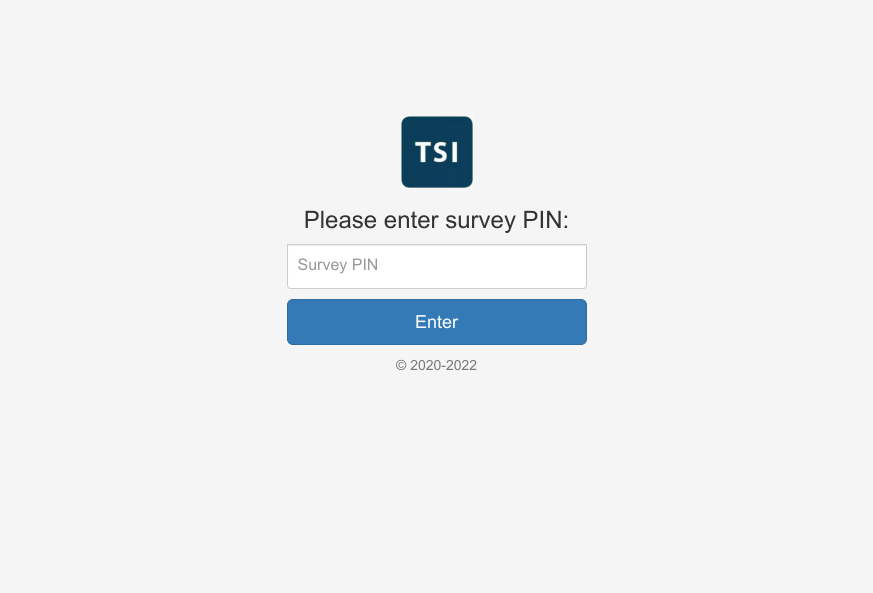
\includegraphics[width=0.80\textwidth]{img/pinscreen.png}}
	\caption{Main screen}
\end{figure}
Once a PIN is entered, user will be bought to the survey screen. If survey is open then user will be able to press on the different answer options. When the survey is over, it will be possible to go back and forth between the questions and to see the valid answers to them, if there is one.
\begin{figure}[H]
	\centering
	\fbox{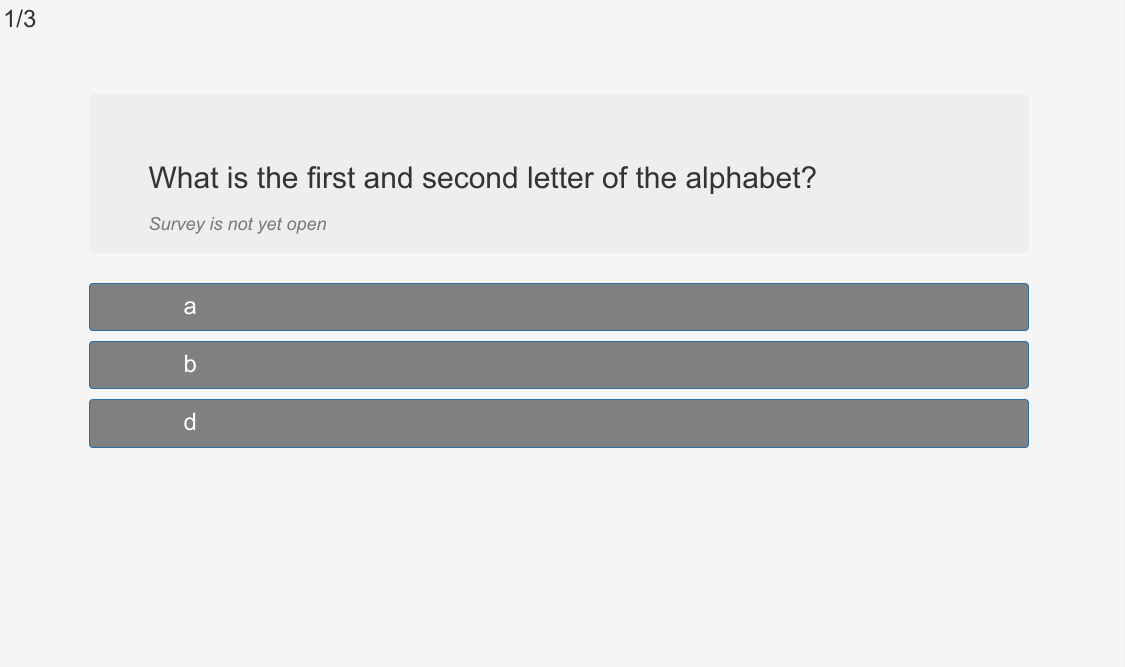
\includegraphics[width=0.80\textwidth]{img/surveyscreen.png}}
	\caption{Survey screen}
\end{figure}
\subsubsection{Survey entity model}
As mentioned before, no data is saved or persisted to any form of database, however to work with the data in a convenient manner it is still structured into some kind of object model. Overall there are 4 model related classes. The first being the \codeword{Item} class.
\begin{figure}[H]
	\centering
	\begin{minted}{python} 
class Item:

    def __init__(self):
        self.id = next(idGenerator)
        self.creationdatetime = datetime.now(tz.gettz("Europe/Riga"))
        self.viewtime = self.creationdatetime.strftime("%c")
	\end{minted}
	\caption{Item class implementation}
\end{figure}
Item class is used as the parent class for the following entity classes. It defines some simple fields that every entity should have.
\begin{figure}[H]
	\centering
	\begin{minted}{python} 
class Presentation(Item):

    def __init__(self, name: str):
        super().__init__()
        self.name = name
        self.surveys = []
        presentations[self.id] = self

    def add_survey(self, s):
        self.surveys.append(s)
	\end{minted}
	\caption{Presentation class implementation}
\end{figure}
The presentation entity is used to represent an ongoing presentation, and it encapsulates all of surveys that happen in it. There are also the \codeword{Survey} and \codeword{SurveyQuestion} entities that store all the information regarding the survey.
\subsubsection{Django HTML templating}
The Django framework provides the creatively named Django Template Language (DTL) for creating HTML templates. All of the screens were written and implemented with it. DTL syntax is fairly simplistic. It was designed to help express presentation and not program logic, making it impossible to just directly execute python expressions with it. Though it does provide tags that function similarly to some programming constructs \citep{djangoDev} which includes for loops, if statements and file importing.
\begin{figure}[H]
	\centering
	\begin{minted}{python} 
<head>
    <title>Nao Presentations</title>
    
</head>
	\end{minted}
	\caption{Example of file importing}
\end{figure}
All HTML pages import the file \enquote{header.html} which contains all the frameworks and libraries used for developing the screens. And also sets the character set to UTF-8 \citep{htmlmanual}. By doing the importing, the following things were done:
\begin{itemize}
	\item jQuery library was imported;
	\item Meta information regarding the viewport and character set was specified;
	\item Bootstrap stylesheet was imported;
	\item Common JS file containing common utility functions was imported.
\end{itemize}
This is a fairly trivial convenience that it afforded with server side rending, and unfortunately it's impossible to do the same with plain HTML without employing some external JS library.
\begin{figure}[H]
	\centering
	\begin{minted}[breaklines,frame=single]{html} 
<meta charset="UTF-8">

<link rel="shortcut icon" type="image/png" href=""/>
<meta name="viewport" content="width=device-width, initial-scale=1">
<link rel="stylesheet" href="https://bootstrapcdn.com/bootstrap/3.4.1/css/bootstrap.min.css">
<link rel="stylesheet" href="">
<script src=""></script>
<script type=" text/javascript" src=""></script>
<script src="https://ajax.googleapis.com/ajax/libs/jquery/3.5.1/jquery.min.js"> </script>
<script src="https://bootstrapcdn.com/bootstrap/3.4.1/js/bootstrap.min.js"> </script>
	\end{minted}
	\caption{Contents of header.html}
\end{figure}
For development of the HTML pages the framework Bootstrap is used and the library jQuery is also utilized. Bootstrap framework mainly being used for stylizing purposes.
\subsubsection{CSS styling}
CSS is a formal language for describing the appearance of a document (web page) written using a markup language (HTML). It can also be applied to any XML document, such as SVG or XUL, though that does not apply for this case.\par
Without CSS, web pages do not have any appeal in their appearance making it a prerequisite for any modern web application. However, CSS is also a very extensive language with much history. The result that being that it's properties interact, often in unexpected ways, and so a certain amount of experience is required to make good use of it. 
In order to side step this barrier the CSS framework Bootstrap was heavily utilized. Bootstrap defines a plethora of CSS classes for all kinds of situations that can be used in the desired HTML pages. For example, the class \codeword{jumbotron} for showcasing hero unit style content.
\begin{figure}[H]
	\centering
	\begin{minted}[breaklines,frame=single]{html} 
<div class="jumbotron">
    <h1>Ongoing NAO presentations:</h1>
</div>
	\end{minted}
	\caption{Example use of bootstrap class}
\end{figure}
The use of bootstrap enables to develop web pages that work across many different devices, including mobile ones \citep{bootstrap}.\par
A generally simplistic design was made for all the pages. Blueish colors are used everywhere due it being a generally neutral color and main color for the TTI university. The only exception being when showing correct and incorrect question options, where green is used indicate a valid option, and red for an invalid one.\par
\subsection{Final class diagram}
During the development phase, many changes were made to the class diagram resulting in a object model very different from what was initially imagined.
\begin{figure}[H]
	\centering
	\begin{plantuml}
@startuml
class Presentation {
	presentation_id
	filesystem_path
	com_presentation_object
	com_slide_show_object
	ongoing_events
	+handle_event()
	-open_presentation()
}

interface TextProcessor {
	+process()
}

class CharacterNormalizer implements TextProcessor {
	+process()
}

class DuplicateSpaceRemover implements TextProcessor {
	+process()
}

class XmlTranslator implements TextProcessor {
	+process() 
}


class TextTranslationSystem {
	+translate()
}

class SlidePresentationService {
	com_slide_show_object
	translation_system: TextTranslationSystem
	chunk_index
	+read_slide()
	-wait_for_ongoing_events_to_stop()
	-next()
}

class PresentationReadingService {
	stop_reading
	slide_reader: SlideReadingService
	event_handler
	slide_index
	+read_presentation()
	-pause()
	-stop()
	-next_slide()
	-prev_slide()
}

class XmlFinder {
	+find_xml_tag()
	-_get_end_tag()
	-_get_tag_finder()
	-_replace()
	-_find_tag()
	-_is_singular()
	-_is_valid_end_tag()
}

class XmlTag {
	+is_singular()
	+is_closed()
	+attributes()
	+start_tag()
	+end_tag()
	+content()
	+child_tags()
	+get_child_tag()
	+get_child_tag_content()
}

interface Callable {
	+__call__()
}

class BehaviorActionEvent implements Callable {
	+__call__()
}

class MediaPresentationEvent implements Callable {
	+__call__()
	-_get_media_shape()
}

class SurveyEvent implements Callable {
	+__call__()
}

class EventWrapper {
	+execute_event()
	+to_string()
	-_get_execution_function()
}

class ComThread {
	+start()
}

PresentationReadingService --o Presentation
SlidePresentationService --o Presentation
TextTranslationSystem --o Presentation


PresentationReadingService --> SlidePresentationService
SlidePresentationService --> TextTranslationSystem
CharacterNormalizer -up-* TextTranslationSystem
DuplicateSpaceRemover -up-* TextTranslationSystem
XmlTranslator -up-* TextTranslationSystem
XmlTranslator --> XmlTag
XmlTag -> XmlFinder
XmlFinder -> XmlTag
BehaviorActionEvent --* SlidePresentationService
MediaPresentationEvent --* SlidePresentationService
SurveyEvent --* SlidePresentationService
EventWrapper --* SlidePresentationService
ComThread --* EventWrapper

@enduml
	\end{plantuml}
	\caption{Final class diagram}
\end{figure}
There are many reasons for this happening. During development certain technical aspects, for example, relating to COM object usage, forced the introduction of more classes to abstract away some technicalities.
\subsection{Code metrics}
In order to quantifiably express the quality and maintainability of the code base, some code metrics have been calculated, by utilizing the python utility \codeword{radon}.
\begin{figure}[H]
	\centering
	\begin{minted}{python} 
161 blocks (classes, functions, methods) analyzed.
Average complexity: A (1.77639751553)
	\end{minted}
	\caption{Total average cyclomatic complexity for presentation controller}
\end{figure}
As a matter of fact, the cyclomatic complexity does not exceed "5" in the entire presentation controller project. One of most cyclomatically complicated functions being the \codeword{\_get\_end\_tag} function inside the \codeword{XmlFinder} class.
\begin{figure}[H]
	\begin{minted}[fontsize=\footnotesize,baselinestretch=1,frame=single]{python} 
    def _get_end_tag(self, stag, tag_finder):
        stag_name = XmlTag(stag).name
        num_to_find = 1
        l, r, tag = None, None, None
        while num_to_find > 0:
            l, r, tag = next(tag_finder)
            if self._is_valid_end_tag(stag, tag):
                num_to_find -= 1
            elif XmlTag(tag).name == stag_name and not self._is_singular(tag):
                num_to_find += 1
        return l, r, tag
	\end{minted}
	\caption{Method with highest cyclomatic complexity}
\end{figure}
In addition, to guage the maintainability of the code base it's \enquote{maintainability index} has been calculated, which shows an overall mixed image.
\begin{itemize}[noitemsep,topsep=1pt]
	\item args.py - A (100.00);
	\item getbehaviours.py - A (100.00);
	\item slidepresentationservice.py - A (53.27);
	\item constants.py - A (100.00);
	\item services.py - A (65.75);
	\item preader.py - A (48.54);
	\item events/event.py - A (47.31);
	\item events/mediapresentationevent.py - A (64.46);
	\item events/surveyevent.py - A (69.72);
	\item events/behavioractionevent.py - A (100.00);
	\item translation/texttranslator.py - A (100.00);
	\item naoxml/xmlfinder.py - A (46.95);
	\item naoxml/xmltag.py - A (35.63);
	\item naoxml/xmlexceptions.py - A (100.00);
	\item naoxml/xmltagvalidator.py - A (76.32);
	\item naoxml/xmltranslator.py - A (32.94);
	\item web/\_webservice.py - A (100.00);
	\item web/webinterface.py - A (57.99);
	\item comthread.py - A (100.00);
	\item general.py - A (68.20);
	\item presentation.py - A (61.48);
	\item survey/survey.py - A (83.43);
	\item main.py - A (74.31).
\end{itemize}\par
The \enquote{maintainability index} is a code metric that measures how maintainable (easy to support and change) source code is. The maintainability index is calculated with a factored formula consisting of Cyclomatic Complexity, SLOC (Source Lines Of Code) and Halstead volume. It is used in several automated software metric tools, including the Microsoft Visual Studio integrated development environment, which uses a shifted scale (0 to 100) derivative. \citep{metrics}
\section{Testing}
In terms of testing, not much of it could be done for the development of the presentation tool suite. Since the largest part of the tool suite is the presentation controller, which requires the use of external resources like the survey conductor and Nao robot, it is not possible to write proper integration tests for it. So testing was mainly done through the use of unit tests and manual labor. The only exception being the survey conductor which is not overly dependent of external resources.
\subsection{Manual testing}
Manual testing was conducted by setting up an environment akin to that of production. Nao robot was set up. Survey conductor was deployed in the cloud and an example presentation was created. This example presentation made use of almost all the created tags, and utilized embedded video/audio.\par
While testing, there some noted cases of errors/exceptions being raised in some apparently random cases at which point it was deemed that the execution process for the presentation controller is volatile and none deterministic. The cause of this was not clear, but after some investigation was deduced to most likely be a race condition somewhere within the Nao SDK library. So to mitigate potential future issue, most of the manual testing came down to replaying the same presentation over and over again until some error showed up and then tracing that error and finding it's cause.\par
\subsection{Automation testing}
Since the Survey Conductor, is not reliant on the presence of Nao or the availability of any external web services, it's testing could be automated to certain extent. For this, Selenium WebDriver was utilized.
Selenium WebDriver is primarily a set of libraries for various programming languages. These libraries are used to send HTTP requests to the driver (hence the name WebDriver), using the JsonWireProtocol protocol, which indicate the action that the browser should perform within the current session. Examples of such commands can be commands for finding elements by a locator, following links, parsing the text of a page/element, pressing buttons, or following links on a website page \citep{selenium, selenium2}.\par
There are both official bindings of the library to popular programming languages, and amateur ones. For example, the PHP language support library is not official and is being developed by Facebook. But in this case the Python bindings were used. As such, all the automation tests were written in Python.\par
Whenever any noteworthy changes were made to the survey conductor, the automation tests would be launched and if any errors were encountered, it would be investigated and resolved.
\subsection{Unit testing}
Unit testing is the process in programming that allows to check the correctness of individual modules of the source code.
The idea is to write tests for every non-trivial function or method. This allows to quickly check whether the next change in the code has led to regression, that is, to the appearance of errors in the already tested parts of the program, and also facilitate the detection and elimination of such errors. For example, you can update the library used in the project to the current version at any time by running tests and identifying incompatibilities.\par
Writing Unit tests in python is a simple affair with PyUnit, a Python port of JUnit. 
Unit tests were written for all of components that could be executed in some form of isolation:
\begin{itemize}
	\item Survey XML to Object mapping;
	\item XML validation;
	\item Notes text translation.
\end{itemize}
To create a test case, one simply has to provide a class that inherits from the \codeword{unittest.TestCase} class, which provides the test routines and also hooks for making each routine and cleaning up after them.\par
Most of these unit tests operate in simple black box manner. A certain input is given, and a certain output is expected. Naturally, if an unexpected exception occurs and the returned output does not match what was expected, the unit test as a whole fails.
\begin{figure}[H]
	\centering
	\begin{minted}[breaklines]{python} 
class MockStartMedia:

    def to_string(self):
        # Event("startmedia", MediaPresentationEvent(), presentation, com_context)
        return " $wait=1 $event=startmedia "


class MockPresentation:
    def __init__(self):
        self.surveys = {}
        self.event_map = {'startmedia': MockStartMedia()}


class TestTranslator(unittest.TestCase):

    def test_translation(self):
        txt = """..."""
        result = TextTranslationSystem(MockPresentation()).translate(txt)
        expected = r"""..."""
        self.assertEquals(result, expected)

	\end{minted}
	\caption{Unit test for notes text translation}
\end{figure}
\addcontentsline{toc}{section}{Conclusion}
\section*{\centering Conclusion}
To conclude, all the main components of the Nao presentation tool suite have been implemented to a varying degree of success. The presentation controller successfully opens a presentation, autonomously goes through and sends commands to Nao to speak the required words.
The survey conductor establishes a web API by which the presentation controller can create and start surveys. The survey conductor also provides a rather simple and intuitive UX for doing these surveys.
\par
While writing the presentation controller some of the written components could be considered redundant. All parts relating to XML processing were manually implemented. XML parsing could have been achieved with the use of the python library \enquote{Beautiful Soup}.
The process of mapping the XML data to object and then later to JSON could have been skipped, by simply using the library \enquote{xmltodict}. XML validation could have also been done by using the library \enquote{lxml} and writing up an XSD (XML Schema Definition) file.\par
Regarding COM, it would have been correct to read more on the subject before utilizing them so much. Initially, it was unknown that COM objects could be used across different threads, so a system marshalling and unmarshalling was implemented to make it possible. This system was later entirely thrown out when MTAs were discovered.\par
While writing the survey conductor many different endpoints were written.
\begin{itemize}
	\item endpoint to manually go to next/previous question;
	\item endpoint to update a survey questions;
	\item endpoint to open/close a survey;
	\item endpoint to get the answer correctness ratio;
	\item endpoint to delete all presentations and surveys.
\end{itemize}
%\begin{figure}[H]
%	\centering
%	\begin{minted}[fontsize=\footnotesize,baselinestretch=1,frame=single]{python} 
%urlpatterns = [
%    path('admin/', admin.site.urls),
%    path('', app.views.pin_page),
%    path('presentations', app.views.index),
%    path('create/presentation', app.views.create_presentation),
%    path('presentation/<int:pid>/create/survey', app.views.create_survey),
%    path('survey/<int:sid>', app.views.get_survey),
%    path('update/survey/<int:sid>', app.views.update_survey),
%    path('open/survey/<int:sid>', app.views.open_survey),
%    path('survey/<int:sid>/next', app.views.survey_next),
%    path('survey/<int:sid>/prev', app.views.survey_prev),
%    path('survey/status/<int:sid>', app.views.get_survey_status),
%    path('survey/pin/<str:pin>', app.views.get_survey_by_pin),
%    path('view/presentation/<int:pid>', app.views.presentation_page),
%    path('view/survey/<int:sid>', app.views.survey_page),
%    path('answer/survey/<int:qid>', app.views.answer_survey_question),
%    path('score/user/<int:sid>', app.views.user_score),
%    path('score/survey/<int:sid>', app.views.survey_score),
%    path('delete/presentation/<int:pid>', app.views.delete_presentation),
%    path('delete/all', app.views.clear_data),
%    path('favicon.ico', app.views.favicon)
%]
%	\end{minted}
%	\caption{Survey conductor endpoints}
%\end{figure}
Many of these endpoints are not utilized in integration with the survey conductor because requirements were not properly defined from the beginning leading to a disorganized API design. The endpoints that allow manual manipulation of the survey are not used because all of the operations were offloaded to the survey conductor making the survey execution process autonomous from the presentation controller.
In addition, the use of models and class entities is questionable. Since the surveys are not saved anywhere, there is no explicit reason for them to be defined as a class and mapped from JSON to a class instance. 
Theoretically, it could have been executed differently, by simply validating the received JSON, converting it to a dictionary and get the required fields from it as necessary. Albeit, such an approach would probably leave not much room for future expansion.
Nonetheless, in the resulting work product there are two different class definitions of the survey class, which could have been mitigated by getting rid of one, or perhaps even both.\par
Most of the above-mentioned inefficiencies came to be for only a couple of reasons, which could have been mitigated at the very start if the appropriate steps were taken.
\begin{itemize}
	\item Poorly defined initial application requirements;
	\item Avoidance of 3rd party library solutions;
	\item Lack of foreknowledge regarding COM.
\end{itemize}
%\nocite{*}

\addcontentsline{toc}{section}{Reference List}
\bibliography{refs.bib} % Entries are in the refs.bib file
\addcontentsline{toc}{section}{Appendix}

%\newcommand{\myappendix}[2]{}}

\clearpage
\vspace*{\fill}
\begin{quote} 
\centering 
\large \textbf{APPENDIX}
\end{quote}
\vfill % equivalent to \vspace{\fill}
\clearpage
\counterwithout{figure}{section}
\setcounter{figure}{0}

\captionsetup {
    format=customappendix,%
    labelformat=customappendix,%
    labelsep=custom
}

\renewcommand\mylstcaption{Example listing of code}

\newcounter{appcount}
\setcounter{appcount}{1}

%\begin{mdlisting}
%\begin{center} \textbf{Appendix \arabic{appcount}}\\ ./args.py \end{center}
%\lstinputlisting[language=python,basicstyle=\footnotesize]{/home/drewman/test/Nao-PPTX/src/args.py}
%\end{mdlisting}
%\stepcounter{appcount}

\begin{mdlisting}
\begin{center} \textbf{Appendix \arabic{appcount}}\\ ./slidepresentationservice.py \end{center}
\lstinputlisting[language=python,basicstyle=\footnotesize]{/home/drewman/test/Nao-PPTX/src/slidepresentationservice.py}
\end{mdlisting}
\stepcounter{appcount}

%\begin{mdlisting}
%\begin{center} \textbf{Appendix \arabic{appcount}}\\ ./services.py \end{center}
%\lstinputlisting,basicstyle=\footnotesize[language=python]{/home/drewman/test/Nao-PPTX/src/services.py}
%\end{mdlisting}
%\stepcounter{appcount}

\begin{mdlisting}
\begin{center} \textbf{Appendix \arabic{appcount}}\\ ./preader.py \end{center}
\lstinputlisting[language=python,basicstyle=\footnotesize]{/home/drewman/test/Nao-PPTX/src/preader.py}
\end{mdlisting}
\stepcounter{appcount}

\begin{mdlisting}
\begin{center} \textbf{Appendix \arabic{appcount}}\\ ./events/mediapresentationevent.py \end{center}
\lstinputlisting[language=python,basicstyle=\footnotesize]{/home/drewman/test/Nao-PPTX/src/events/mediapresentationevent.py}
\end{mdlisting}
\stepcounter{appcount}

\begin{mdlisting}
\begin{center} \textbf{Appendix \arabic{appcount}}\\ ./events/surveyevent.py \end{center}
\lstinputlisting[language=python,basicstyle=\footnotesize]{/home/drewman/test/Nao-PPTX/src/events/surveyevent.py}
\end{mdlisting}
\stepcounter{appcount}

\begin{mdlisting}
\begin{center} \textbf{Appendix \arabic{appcount}}\\ ./events/behavioractionevent.py \end{center}
\lstinputlisting[language=python,basicstyle=\footnotesize]{/home/drewman/test/Nao-PPTX/src/events/behavioractionevent.py}
\end{mdlisting}
\stepcounter{appcount}


\begin{mdlisting}
\begin{center} \textbf{Appendix \arabic{appcount}}\\ ./translation/texttranslator.py \end{center}
\lstinputlisting[language=python,basicstyle=\footnotesize]{/home/drewman/test/Nao-PPTX/src/translation/texttranslator.py}
\end{mdlisting}
\stepcounter{appcount}


%\begin{mdlisting}
%\begin{center} \textbf{Appendix \arabic{appcount}}\\ ./naoxml/xmlfinder.py \end{center}
%\lstinputlisting,basicstyle=\footnotesize[language=python]{/home/drewman/test/Nao-PPTX/src/naoxml/xmlfinder.py}
%\end{mdlisting}
%\stepcounter{appcount}

%\begin{mdlisting}
%\begin{center} \textbf{Appendix \arabic{appcount}}\\ ./naoxml/xmltag.py \end{center}
%\lstinputlisting[language=python,basicstyle=\footnotesize]{/home/drewman/test/Nao-PPTX/src/naoxml/xmltag.py}
%\end{mdlisting}
%\stepcounter{appcount}

%\begin{mdlisting}
%\begin{center} \textbf{Appendix \arabic{appcount}}\\ ./naoxml/xmltranslator.py \end{center}
%\lstinputlisting[language=python,basicstyle=\footnotesize]{/home/drewman/test/Nao-PPTX/src/naoxml/xmltranslator.py}
%\end{mdlisting}
%\stepcounter{appcount}

\begin{mdlisting}
\begin{center} \textbf{Appendix \arabic{appcount}}\\ ./comthread.py \end{center}
\lstinputlisting[language=python,basicstyle=\footnotesize]{/home/drewman/test/Nao-PPTX/src/comthread.py}
\end{mdlisting}
\stepcounter{appcount}

%\begin{mdlisting}
%\begin{center} \textbf{Appendix \arabic{appcount}}\\ ./general.py \end{center}
%\lstinputlisting,basicstyle=\footnotesize[language=python]{/home/drewman/test/Nao-PPTX/src/general.py}
%\end{mdlisting}
%\stepcounter{appcount}

\begin{mdlisting}
\begin{center} \textbf{Appendix \arabic{appcount}}\\ ./presentation.py \end{center}
\lstinputlisting[language=python,basicstyle=\footnotesize]{/home/drewman/test/Nao-PPTX/src/presentation.py}
\end{mdlisting}
\stepcounter{appcount}

%\begin{mdlisting}
%\begin{center} \textbf{Appendix \arabic{appcount}}\\ ./survey/survey.py \end{center}
%\lstinputlisting,basicstyle=\footnotesize[language=python]{/home/drewman/test/Nao-PPTX/src/survey/survey.py}
%\end{mdlisting}
%\stepcounter{appcount}

%\begin{mdlisting}
%\begin{center} \textbf{Appendix \arabic{appcount}}\\ ./main.py \end{center}
%\lstinputlisting,basicstyle=\footnotesize[language=python]{/home/drewman/test/Nao-PPTX/src/main.py}
%\end{mdlisting}
%\stepcounter{appcount}


\end{document}
